\documentclass[a4paper,12pt]{article}
\usepackage{graphicx}
\usepackage[UTF8]{ctex}
\usepackage{fontspec}
\usepackage{booktabs}
\usepackage{float}%浮动体
\usepackage{amsmath,amssymb}
\usepackage{fancyhdr}
%\usepackage{xcolor}
\usepackage{colortbl}
\usepackage{geometry}
\geometry{top=2cm,bottom=2cm,left=1cm,right=1cm}
\begin{document}
	\begin{figure}[H]
	\begin{center}
		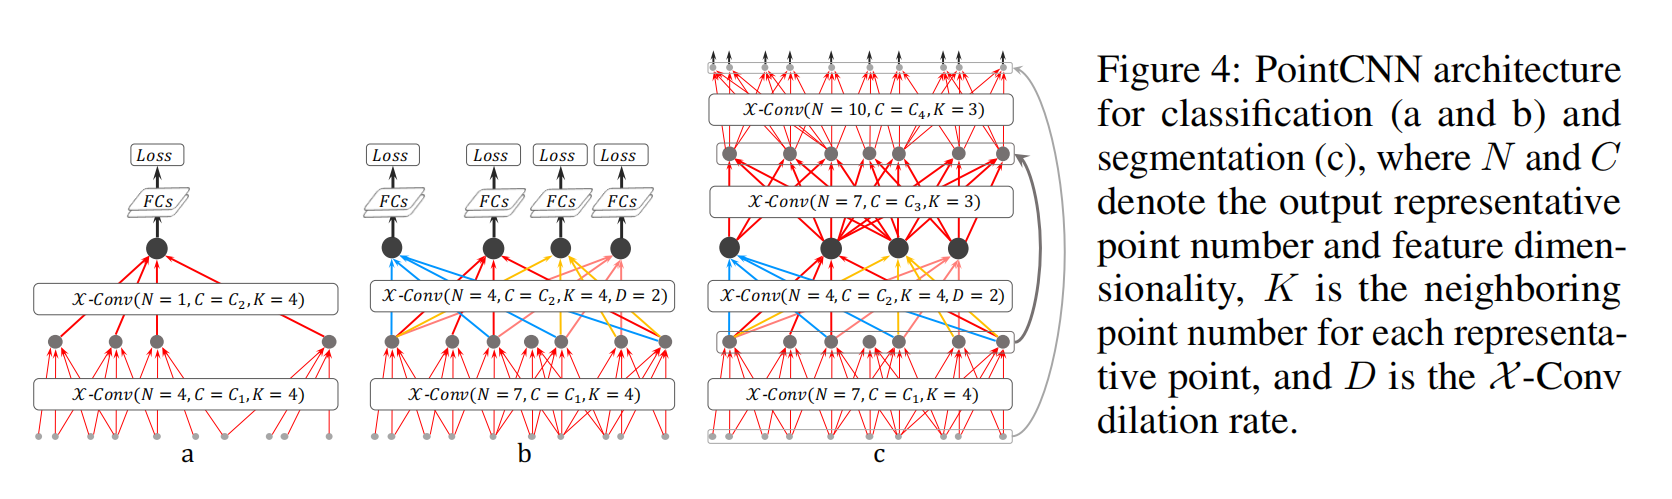
\includegraphics[width=0.9\textwidth]{img/PointCNN.png} 
		\caption{PointCNN}
	\end{center}
\end{figure}

\textbf{X-transformation}:
\begin{itemize}
	\item 给点的特征进行赋权重
	\item 将点转置到一个潜在的标准顺序
\end{itemize}

	\begin{figure}[H]
		\begin{center}
			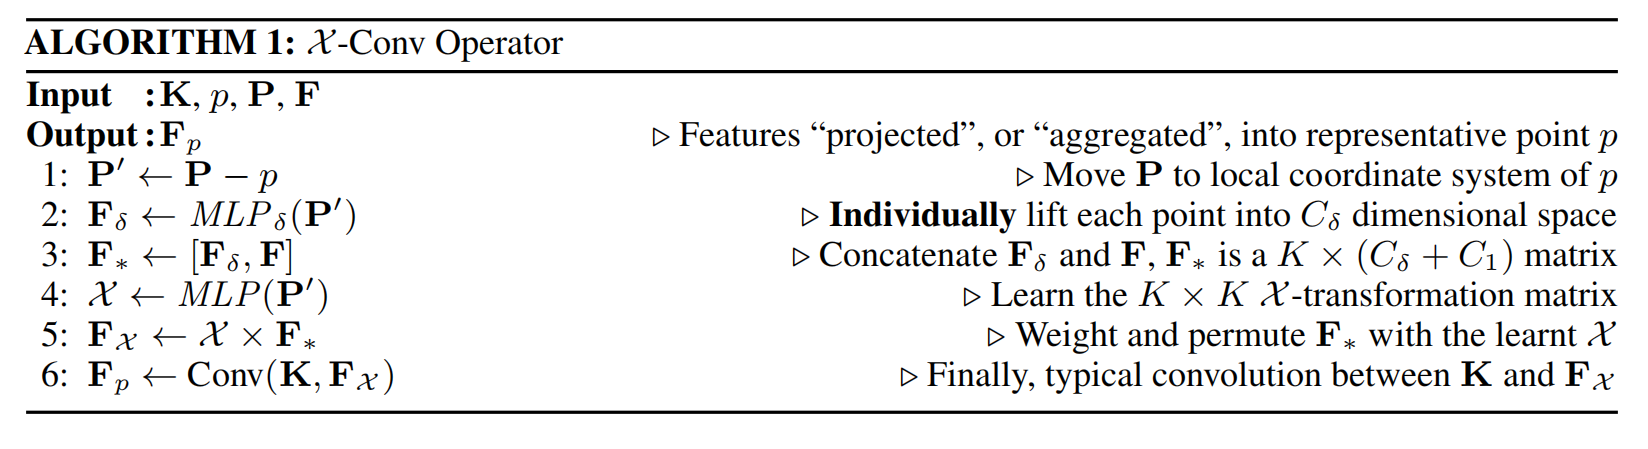
\includegraphics[width=0.9\textwidth]{img/PointCNN_ALG.png} 
			\caption{X-conv}
		\end{center}
	\end{figure}

$$
\mathbf{F}_{p}=\mathcal{X}-\operatorname{Conv}(\mathbf{K}, p, \mathbf{P}, \mathbf{F})=\operatorname{Conv}\left(\mathbf{K}, M L P(\mathbf{P}-p) \times\left[M L P_{\delta}(\mathbf{P}-p), \mathbf{F}\right]\right)
$$


\paragraph{分类任务}
有两种网络,分别对应图1的a,b。b在保留相同卷积深度的基础上,加入了卷积dilation,增加了感受域,但未卷积核的大小。
\paragraph{语义分割} 在特征提取之后,进行"反卷积",还原回最初的点的个数。

\end{document}